% automatically generated document using lt2circuiTikz
\documentclass[tikz,margin={2pt 2pt 2pt 2pt}]{standalone}
\usepackage[compatibility,siunitx,  americanvoltages, americancurrents, europeanresistors, europeaninductors, americanports,%
  straightlabels, fetbodydiode, straightvoltages]{circuitikz}
\usepackage{tikz,amsmath, amssymb,bm,color,pgfkeys,siunitx,ifthen,ulem}
\usepackage{pgfplots}
\pgfplotsset{compat=1.14}
\usetikzlibrary{shapes,arrows}
%\usepackage{agaramondc}					% Adobe Garamond, custom shape
%\renewcommand{\shapedefault}{rtl} % rtl: roman tabular lining

\makeatletter

%% bandstop filter (adapted from highpass)
\pgfcircdeclarebipole{}{\ctikzvalof{bipoles/highpass/width}}{*bandstop}{\ctikzvalof{bipoles/highpass/width}}{\ctikzvalof{bipoles/highpass/width}}{
	\pgf@circ@res@step = \ctikzvalof{bipoles/highpass/width}\pgf@circ@Rlen
	\divide \pgf@circ@res@step by 2
	
	\pgfpathmoveto{\pgfpoint{\pgf@circ@res@left}{\pgf@circ@res@zero}}
	\pgf@circ@res@other = \pgf@circ@res@left
	\advance\pgf@circ@res@other by \pgf@circ@res@step 
	
	\ifpgf@circuit@dashed
	\pgfsetdash{{0.1cm}{0.1cm}}{0cm} 
	\fi	
	
	% draw outer box
	\pgfsetlinewidth{\pgfkeysvalueof{/tikz/circuitikz/bipoles/thickness}\pgfstartlinewidth}
	\pgfpathrectanglecorners{\pgfpoint{\pgf@circ@res@left}{\pgf@circ@res@up}}{\pgfpoint{\pgf@circ@res@right}{\pgf@circ@res@down}}
	\pgfusepath{draw}
	
	\ifpgf@circuit@inputarrow
	{
		\advance \pgf@circ@res@left by -.5\pgfkeysvalueof{/tikz/circuitikz/bipoles/thickness}\pgfstartlinewidth
		\pgftransformshift{\pgfpoint{\pgf@circ@res@left}{0pt}}
		\pgfnode{inputarrow}{tip}{}{pgf@inputarrow}{\pgfusepath{fill}}
	}
	\fi
	
	% rotate inner symbol
	\def\pgfcircmathresult{\expandafter\pgf@circ@stripdecimals\pgf@circ@direction\pgf@nil}
	\ifnum \pgfcircmathresult > 45 \ifnum \pgfcircmathresult < 135
	\pgftransformrotate{270}
	\fi\fi
	\ifnum \pgfcircmathresult > 134 \ifnum \pgfcircmathresult < 225  % 134 degree, because >= 135 is not possible
	\pgftransformrotate{180}
	\fi\fi
	\ifnum \pgfcircmathresult > 224 \ifnum \pgfcircmathresult < 315
	\pgftransformrotate{90}
	\fi\fi
	
	% draw inner symbol
	\pgfsetdash{}{0pt}	% always draw solid line for inner symbol
	\pgfsetarrows{-} %never draw arrows
	\pgfsetlinewidth{\pgfstartlinewidth}
	\pgfpathmoveto{\pgfpoint{-0.5\pgf@circ@res@step}{0.5\pgf@circ@res@step}}
	\pgfpathsine{\pgfpoint{.25\pgf@circ@res@step}{.25\pgf@circ@res@step}}
	\pgfpathcosine{\pgfpoint{.25\pgf@circ@res@step}{-.25\pgf@circ@res@step}}
	\pgfpathsine{\pgfpoint{.25\pgf@circ@res@step}{-.25\pgf@circ@res@step}}
	\pgfpathcosine{\pgfpoint{.25\pgf@circ@res@step}{.25\pgf@circ@res@step}}
	\pgfusepath{draw}
	
	\pgfpathmoveto{\pgfpoint{-0.5\pgf@circ@res@step}{0}}
	\pgfpathsine{\pgfpoint{.25\pgf@circ@res@step}{.25\pgf@circ@res@step}}
	\pgfpathcosine{\pgfpoint{.25\pgf@circ@res@step}{-.25\pgf@circ@res@step}}
	\pgfpathsine{\pgfpoint{.25\pgf@circ@res@step}{-.25\pgf@circ@res@step}}
	\pgfpathcosine{\pgfpoint{.25\pgf@circ@res@step}{.25\pgf@circ@res@step}}
	\pgfusepath{draw}
	\pgfpathmoveto{\pgfpoint{-0.15\pgf@circ@res@step}{-0.15\pgf@circ@res@step}}
	\pgfpathlineto{\pgfpoint{0.15\pgf@circ@res@step}{0.15\pgf@circ@res@step}}
	\pgfusepath{draw}
	
	\pgfpathmoveto{\pgfpoint{-0.5\pgf@circ@res@step}{-0.5\pgf@circ@res@step}}
	\pgfpathsine{\pgfpoint{.25\pgf@circ@res@step}{.25\pgf@circ@res@step}}
	\pgfpathcosine{\pgfpoint{.25\pgf@circ@res@step}{-.25\pgf@circ@res@step}}
	\pgfpathsine{\pgfpoint{.25\pgf@circ@res@step}{-.25\pgf@circ@res@step}}
	\pgfpathcosine{\pgfpoint{.25\pgf@circ@res@step}{.25\pgf@circ@res@step}}
	\pgfusepath{draw}
	%	\pgfpathmoveto{\pgfpoint{-0.15\pgf@circ@res@step}{-0.65\pgf@circ@res@step}}
	%	\pgfpathlineto{\pgfpoint{0.15\pgf@circ@res@step}{-0.35\pgf@circ@res@step}}
	%	\pgfusepath{draw}
}

\tikzset{
	*bandstop/.style={\circuitikzbasekey, /tikz/to path=\pgf@circ@*bandstop@path},
}
\def\pgf@circ@*bandstop@path#1{\pgf@circ@bipole@path{*bandstop}{#1}}




\makeatother

\usetikzlibrary{backgrounds,calc,positioning}

\usetikzlibrary{circuits.ee.IEC}
\usetikzlibrary{arrows}


% sym32a style

\ctikzset{tripoles/mos style/arrows}
\ctikzset{
	/tikz/circuitikz/quadpoles/coupler/width=1,%1.3
	/tikz/circuitikz/quadpoles/coupler/height=0.952,%1.3
	/tikz/circuitikz/quadpoles/coupler2/width=1,%1.3
	/tikz/circuitikz/quadpoles/coupler2/height=0.952,%1.3
	/tikz/circuitikz/quadpoles/transformer/width=1.425,%1.5
	/tikz/circuitikz/quadpoles/transformer/height=1.425,%1.5
	/tikz/circuitikz/quadpoles/transformer core/width=1.425,%1.5
	/tikz/circuitikz/quadpoles/transformer core/height=1.425,%1.5
	/tikz/circuitikz/quadpoles/gyrator/width=1.425,%1.5
	/tikz/circuitikz/quadpoles/gyrator/height=1.425,%1.5
	%/tikz/circuitikz/monopoles/tlinestub/width=0.1875,%0.25 no effect!
	/tikz/circuitikz/tripoles/american and port/height=0.95,%.8
	/tikz/circuitikz/tripoles/american nand port/height=0.95,%.8
	/tikz/circuitikz/tripoles/american or port/height=0.95,%.8
	/tikz/circuitikz/tripoles/american nor port/height=0.95,%.8
	/tikz/circuitikz/tripoles/american xor port/height=0.95,%.8
	/tikz/circuitikz/tripoles/american xnor port/height=0.95,%.8
	/tikz/circuitikz/bipoles/tline/height=0.4,%0.3
%	/tikz/circuitikz/bipoles/tline/width=1.2,%0.8
	/tikz/circuitikz/bipoles/diode/height=0.375,%
	/tikz/circuitikz/bipoles/diode/width=0.375,%
	/tikz/circuitikz/bipoles/varcap/height=0.375,%
	/tikz/circuitikz/bipoles/varcap/width=0.375,%
	/tikz/circuitikz/tripoles/triac/height=1.05,%
	/tikz/circuitikz/tripoles/triac/width=0.952,%
	/tikz/circuitikz/tripoles/thyristor/height=1.05,%
	/tikz/circuitikz/tripoles/thyristor/width=0.952,%
	/tikz/circuitikz/tripoles/op amp/height=0.952,%
	/tikz/circuitikz/tripoles/op amp/width=1.2,%
	/tikz/circuitikz/tripoles/op amp/font=\footnotesize,
	/tikz/circuitikz/tripoles/gm amp/height=0.952,% 1.7
	/tikz/circuitikz/tripoles/gm amp/width=1.2,% 1.4
	%	/tikz/circuitikz/tripoles/gm amp/font=\footnotesize,
	/tikz/circuitikz/tripoles/plain amp/height=0.952,% 1.7
	/tikz/circuitikz/tripoles/plain amp/width=1.2,% 1.4
	/tikz/circuitikz/bipoles/resistor/voltage/straight label distance/.initial=.8,
	/tikz/circuitikz/bipoles/generic/voltage/straight label distance/.initial=.8,
	/tikz/circuitikz/bipoles/inductor/voltage/straight label distance/.initial=.8,
	/tikz/circuitikz/bipoles/fullgeneric/voltage/straight label distance/.initial=.8,
	/tikz/circuitikz/bipoles/capacitor/voltage/straight label distance/.initial=1.0,
	/tikz/circuitikz/bipoles/thickness=1.6,
}
\ctikzset{v/.append style={/tikz/european voltages}}

\definecolor{netlabelcolor}{rgb}{0, 0, 0.25}
\definecolor{lttotitextcolor}{rgb}{0, 0.4, 0.25}
\definecolor{lttotidrawcolor}{rgb}{0.6, 0.6, 0.6}
\definecolor{netcolor}{rgb}{0, 0, 0.5}

\pgfkeys{/lt2ti/netlabel/font/.initial= \small}
\pgfkeys{/lt2ti/text/font/.initial= \small}

\pgfkeys{/lt2ti/Net/.style= {netcolor}}
\tikzstyle{dashdotdotted}=[dash pattern=on 3pt off 2pt on \the\pgflinewidth off 2pt on \the\pgflinewidth off 2pt]

\pgfkeys{/lt2ti/VArrow/.style= {->,>=latex}}
\pgfkeys{/lt2ti/SArrow/.style= {->,>=angle 90}}

\begin{document}%
	%\centering%
		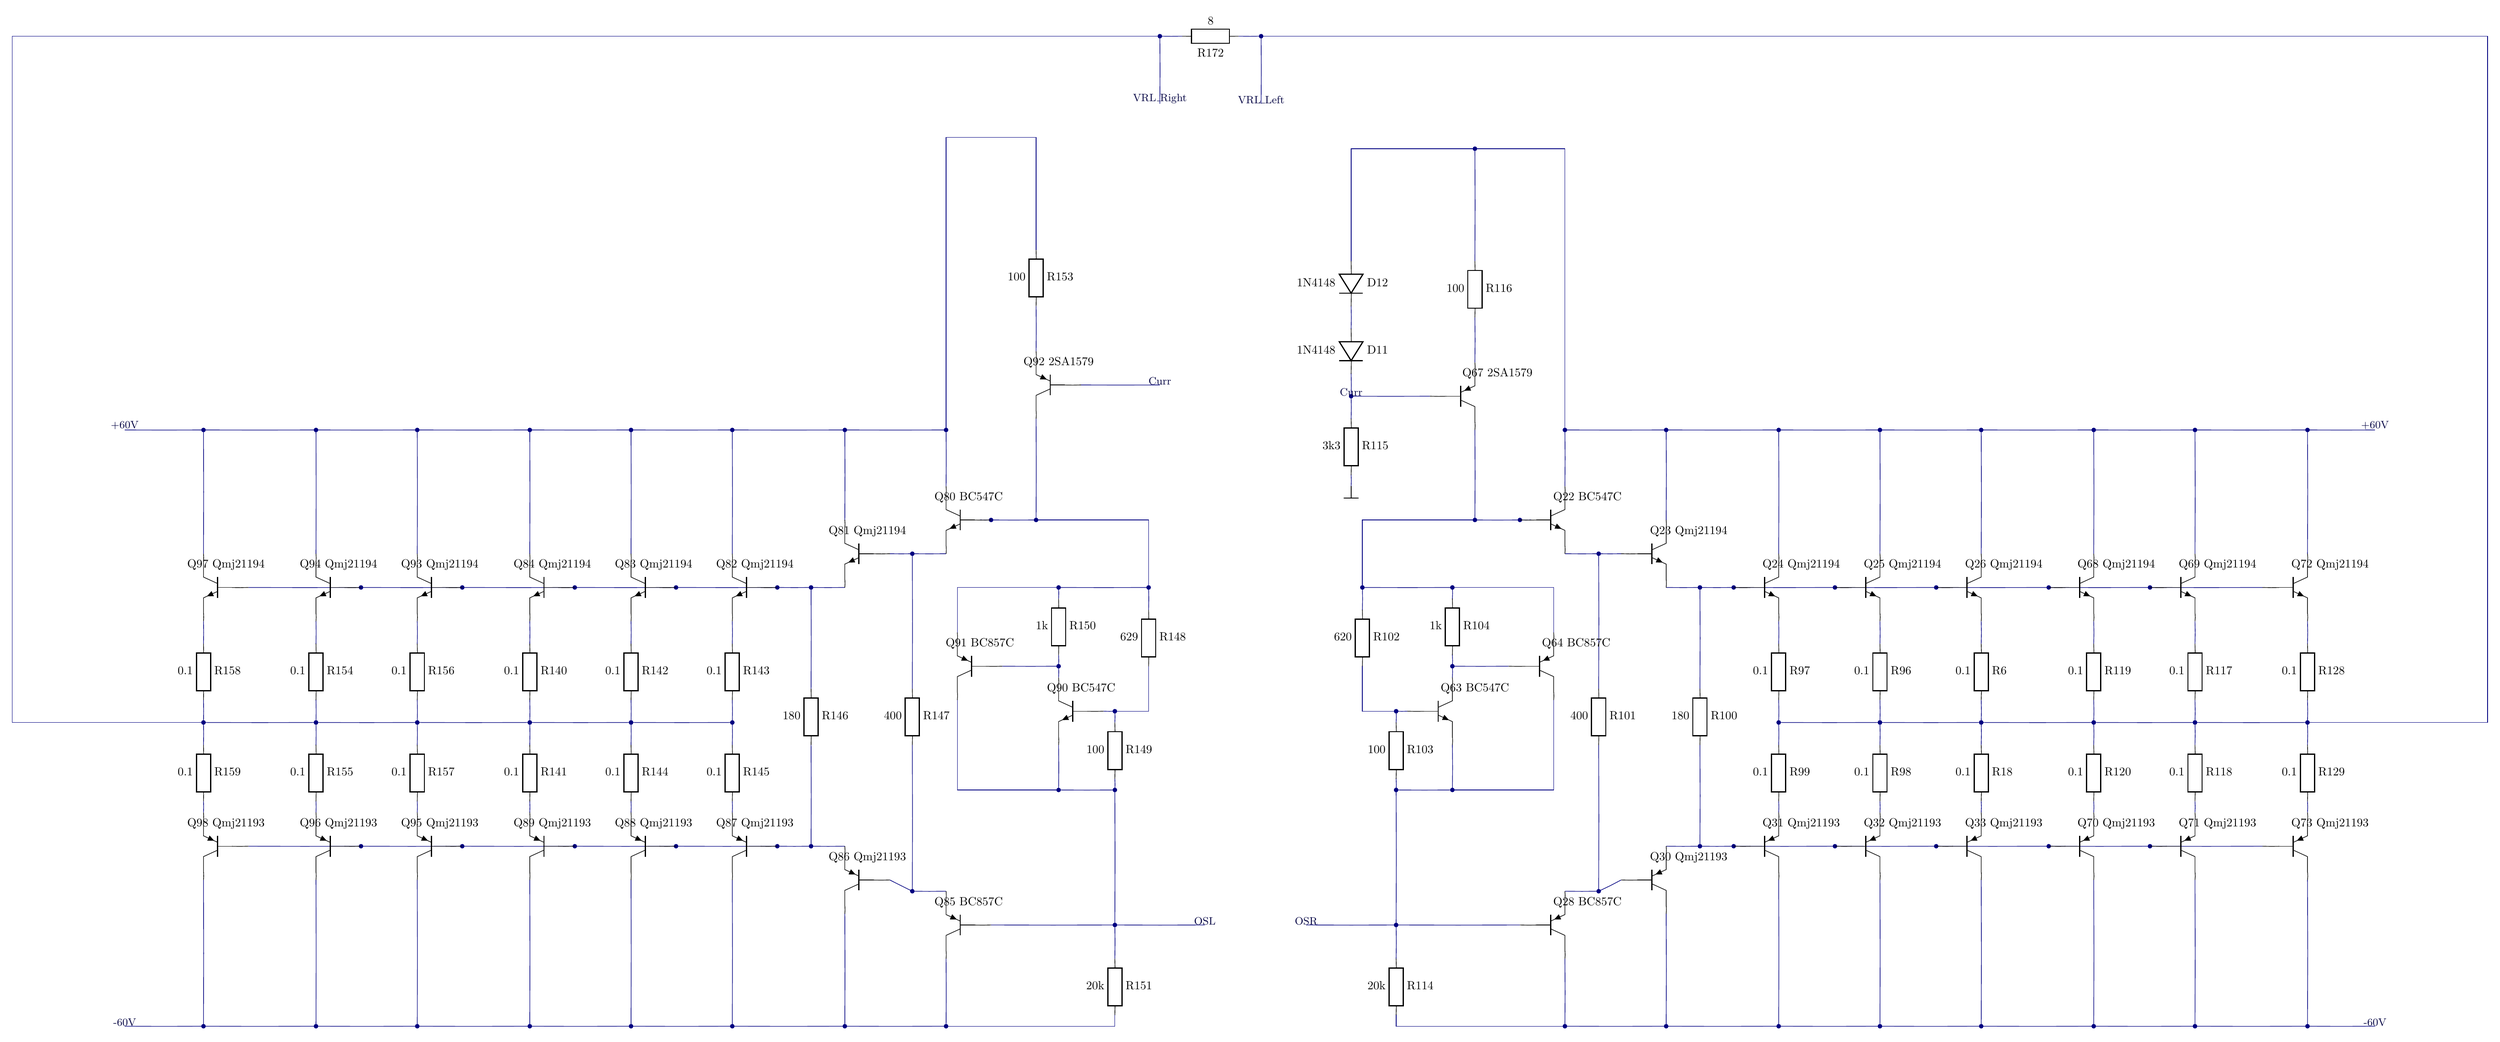
\begin{tikzpicture}[circuit ee IEC, scale=0.6666666667,line width=.5pt]% default: 0.4
	%\tikzstyle{every node}=[font=\small];%
	%\node [draw] at (0.0,0.0) {\pgfkeysvalueof{/tikz/circuitikz/tripoles/op amp/font}};
\draw [/lt2ti/Net](239.5,-140.5)to[*short,-*, color=netcolor] (238.5,-140.5);% wire w4
\draw [/lt2ti/Net](243.0,-140.5)to[*short,*-, color=netcolor] (242.0,-140.5);% wire w5
\draw [/lt2ti/Net](238.5,-143.5)to[*short,-*, color=netcolor] (238.5,-140.5);% wire w7
\draw [/lt2ti/Net](243.0,-143.5)to[*short,-*, color=netcolor] (243.0,-140.5);% wire w8
\draw [/lt2ti/Net](252.5,-145.5)to[*short,*-, color=netcolor] (252.5,-145.5);% wire w10_w13 start
\draw [/lt2ti/Net](247.0,-150.5)to[*short,-, color=netcolor] (247.0,-150.5);% wire w10_w13 end
\draw [/lt2ti/Net](252.5,-145.5) --  (247.0,-145.5) -- (247.0,-150.5); % wire w10_w13 polyline 
\draw [/lt2ti/Net](252.5,-150.5)to[*short,-*, color=netcolor] (252.5,-145.5);% wire w14
\draw [/lt2ti/Net](247.0,-153.5)to[*short,-, color=netcolor] (247.0,-152.5);% wire w15
\draw [/lt2ti/Net](233.0,-154.5)to[*short,-, color=netcolor] (233.0,-152.5);% wire w16
\draw [/lt2ti/Net](252.5,-155.0)to[*short,-, color=netcolor] (252.5,-153.0);% wire w17
\draw [/lt2ti/Net](238.5,-156.0)to[*short,-, color=netcolor] (235.0,-156.0);% wire w18
\draw [/lt2ti/Net](247.0,-156.5)to[*short,*-, color=netcolor] (247.0,-155.5);% wire w19
\draw [/lt2ti/Net](250.5,-156.5)to[*short,-*, color=netcolor] (247.0,-156.5);% wire w20
\draw [/lt2ti/Net](247.0,-157.5)to[*short,-*, color=netcolor] (247.0,-156.5);% wire w21
\draw [/lt2ti/Net](196.0,-158.0)to[*short,*-, color=netcolor] (192.5,-158.0);% wire w22
\draw [/lt2ti/Net](201.0,-158.0)to[*short,*-*, color=netcolor] (196.0,-158.0);% wire w23
\draw [/lt2ti/Net](205.5,-158.0)to[*short,*-*, color=netcolor] (201.0,-158.0);% wire w24
\draw [/lt2ti/Net](210.5,-158.0)to[*short,*-*, color=netcolor] (205.5,-158.0);% wire w25
\draw [/lt2ti/Net](215.0,-158.0)to[*short,*-*, color=netcolor] (210.5,-158.0);% wire w26
\draw [/lt2ti/Net](219.5,-158.0)to[*short,*-*, color=netcolor] (215.0,-158.0);% wire w27
\draw [/lt2ti/Net](224.5,-158.0)to[*short,*-*, color=netcolor] (219.5,-158.0);% wire w28
\draw [/lt2ti/Net](229.0,-158.0)to[*short,*-*, color=netcolor] (224.5,-158.0);% wire w30
\draw [/lt2ti/Net](229.0,-158.0)to[*short,*-, color=netcolor] (229.0,-158.0);% wire w29_w9_w12 start
\draw [/lt2ti/Net](233.0,-150.0)to[*short,-, color=netcolor] (233.0,-150.0);% wire w29_w9_w12 end
\draw [/lt2ti/Net](229.0,-158.0) --  (229.0,-145.0) --  (233.0,-145.0) -- (233.0,-150.0); % wire w29_w9_w12 polyline 
\draw [/lt2ti/Net](256.5,-158.0)to[*short,*-, color=netcolor] (256.5,-158.0);% wire w11_w31 start
\draw [/lt2ti/Net](252.5,-145.5)to[*short,-*, color=netcolor] (252.5,-145.5);% wire w11_w31 end
\draw [/lt2ti/Net](256.5,-158.0) --  (256.5,-145.5) -- (252.5,-145.5); % wire w11_w31 polyline 
\draw [/lt2ti/Net](261.0,-158.0)to[*short,*-*, color=netcolor] (256.5,-158.0);% wire w32
\draw [/lt2ti/Net](266.0,-158.0)to[*short,*-*, color=netcolor] (261.0,-158.0);% wire w33
\draw [/lt2ti/Net](270.5,-158.0)to[*short,*-*, color=netcolor] (266.0,-158.0);% wire w34
\draw [/lt2ti/Net](275.0,-158.0)to[*short,*-*, color=netcolor] (270.5,-158.0);% wire w35
\draw [/lt2ti/Net](280.0,-158.0)to[*short,*-*, color=netcolor] (275.0,-158.0);% wire w36
\draw [/lt2ti/Net](284.5,-158.0)to[*short,*-*, color=netcolor] (280.0,-158.0);% wire w37
\draw [/lt2ti/Net](289.5,-158.0)to[*short,*-*, color=netcolor] (284.5,-158.0);% wire w38
\draw [/lt2ti/Net](292.5,-158.0)to[*short,-*, color=netcolor] (289.5,-158.0);% wire w39
\draw [/lt2ti/Net](229.0,-160.5)to[*short,-*, color=netcolor] (229.0,-158.0);% wire w40
\draw [/lt2ti/Net](247.0,-160.5)to[*short,-, color=netcolor] (247.0,-160.0);% wire w41
\draw [/lt2ti/Net](256.5,-160.5)to[*short,-*, color=netcolor] (256.5,-158.0);% wire w42
\draw [/lt2ti/Net](224.5,-162.0)to[*short,-*, color=netcolor] (224.5,-158.0);% wire w43
\draw [/lt2ti/Net](231.0,-162.0)to[*short,*-, color=netcolor] (230.5,-162.0);% wire w44
\draw [/lt2ti/Net](233.0,-162.0)to[*short,*-, color=netcolor] (233.0,-157.5);% wire w45
\draw [/lt2ti/Net](233.0,-162.0)to[*short,*-*, color=netcolor] (231.0,-162.0);% wire w46
\draw [/lt2ti/Net](252.5,-162.0)to[*short,*-, color=netcolor] (252.5,-158.0);% wire w48
\draw [/lt2ti/Net](252.5,-162.0)to[*short,*-, color=netcolor] (252.5,-162.0);% wire w49_w79 start
\draw [/lt2ti/Net](247.5,-165.0)to[*short,-*, color=netcolor] (247.5,-165.0);% wire w49_w79 end
\draw [/lt2ti/Net](252.5,-162.0) --  (247.5,-162.0) -- (247.5,-165.0); % wire w49_w79 polyline 
\draw [/lt2ti/Net](254.5,-162.0)to[*short,*-*, color=netcolor] (252.5,-162.0);% wire w50
\draw [/lt2ti/Net](255.0,-162.0)to[*short,-*, color=netcolor] (254.5,-162.0);% wire w51
\draw [/lt2ti/Net](261.0,-162.0)to[*short,-*, color=netcolor] (261.0,-158.0);% wire w52
\draw [/lt2ti/Net](196.0,-163.5)to[*short,-*, color=netcolor] (196.0,-158.0);% wire w53
\draw [/lt2ti/Net](201.0,-163.5)to[*short,-*, color=netcolor] (201.0,-158.0);% wire w54
\draw [/lt2ti/Net](205.5,-163.5)to[*short,-*, color=netcolor] (205.5,-158.0);% wire w55
\draw [/lt2ti/Net](210.5,-163.5)to[*short,-*, color=netcolor] (210.5,-158.0);% wire w56
\draw [/lt2ti/Net](215.0,-163.5)to[*short,-*, color=netcolor] (215.0,-158.0);% wire w57
\draw [/lt2ti/Net](219.5,-163.5)to[*short,-*, color=netcolor] (219.5,-158.0);% wire w58
\draw [/lt2ti/Net](227.5,-163.5)to[*short,*-, color=netcolor] (226.5,-163.5);% wire w59
\draw [/lt2ti/Net](229.0,-163.5)to[*short,-*, color=netcolor] (227.5,-163.5);% wire w60
\draw [/lt2ti/Net](258.0,-163.5)to[*short,*-, color=netcolor] (256.5,-163.5);% wire w61
\draw [/lt2ti/Net](259.0,-163.5)to[*short,-*, color=netcolor] (258.0,-163.5);% wire w62
\draw [/lt2ti/Net](266.0,-163.5)to[*short,-*, color=netcolor] (266.0,-158.0);% wire w63
\draw [/lt2ti/Net](270.5,-163.5)to[*short,-*, color=netcolor] (270.5,-158.0);% wire w64
\draw [/lt2ti/Net](275.0,-163.5)to[*short,-*, color=netcolor] (275.0,-158.0);% wire w65
\draw [/lt2ti/Net](280.0,-163.5)to[*short,-*, color=netcolor] (280.0,-158.0);% wire w66
\draw [/lt2ti/Net](284.5,-163.5)to[*short,-*, color=netcolor] (284.5,-158.0);% wire w67
\draw [/lt2ti/Net](289.5,-163.5)to[*short,-*, color=netcolor] (289.5,-158.0);% wire w68
\draw [/lt2ti/Net](203.0,-165.0)to[*short,*-, color=netcolor] (198.0,-165.0);% wire w69
\draw [/lt2ti/Net](207.5,-165.0)to[*short,*-*, color=netcolor] (203.0,-165.0);% wire w70
\draw [/lt2ti/Net](212.5,-165.0)to[*short,*-*, color=netcolor] (207.5,-165.0);% wire w71
\draw [/lt2ti/Net](217.0,-165.0)to[*short,*-*, color=netcolor] (212.5,-165.0);% wire w72
\draw [/lt2ti/Net](221.5,-165.0)to[*short,*-*, color=netcolor] (217.0,-165.0);% wire w73
\draw [/lt2ti/Net](223.0,-165.0)to[*short,*-*, color=netcolor] (221.5,-165.0);% wire w74
\draw [/lt2ti/Net](224.5,-165.0)to[*short,-*, color=netcolor] (223.0,-165.0);% wire w75
\draw [/lt2ti/Net](234.0,-165.0)to[*short,*-, color=netcolor] (234.0,-165.0);% wire w76_w93 start
\draw [/lt2ti/Net](229.5,-167.0)to[*short,-, color=netcolor] (229.5,-167.0);% wire w76_w93 end
\draw [/lt2ti/Net](234.0,-165.0) --  (229.5,-165.0) -- (229.5,-167.0); % wire w76_w93 polyline 
\draw [/lt2ti/Net](238.0,-165.0)to[*short,*-*, color=netcolor] (234.0,-165.0);% wire w78
\draw [/lt2ti/Net](238.0,-165.0)to[*short,*-, color=netcolor] (238.0,-165.0);% wire w47_w77 start
\draw [/lt2ti/Net](233.0,-162.0)to[*short,-*, color=netcolor] (233.0,-162.0);% wire w47_w77 end
\draw [/lt2ti/Net](238.0,-165.0) --  (238.0,-162.0) -- (233.0,-162.0); % wire w47_w77 polyline 
\draw [/lt2ti/Net](251.5,-165.0)to[*short,*-*, color=netcolor] (247.5,-165.0);% wire w80
\draw [/lt2ti/Net](262.5,-165.0)to[*short,*-, color=netcolor] (261.0,-165.0);% wire w82
\draw [/lt2ti/Net](264.0,-165.0)to[*short,*-*, color=netcolor] (262.5,-165.0);% wire w83
\draw [/lt2ti/Net](268.5,-165.0)to[*short,*-*, color=netcolor] (264.0,-165.0);% wire w84
\draw [/lt2ti/Net](273.0,-165.0)to[*short,*-*, color=netcolor] (268.5,-165.0);% wire w85
\draw [/lt2ti/Net](278.0,-165.0)to[*short,*-*, color=netcolor] (273.0,-165.0);% wire w86
\draw [/lt2ti/Net](282.5,-165.0)to[*short,*-*, color=netcolor] (278.0,-165.0);% wire w87
\draw [/lt2ti/Net](287.5,-165.0)to[*short,-*, color=netcolor] (282.5,-165.0);% wire w88
\draw [/lt2ti/Net](234.0,-165.5)to[*short,-*, color=netcolor] (234.0,-165.0);% wire w89
\draw [/lt2ti/Net](251.5,-165.5)to[*short,-*, color=netcolor] (251.5,-165.0);% wire w90
\draw [/lt2ti/Net](238.0,-166.0)to[*short,-*, color=netcolor] (238.0,-165.0);% wire w91
\draw [/lt2ti/Net](247.5,-166.0)to[*short,-*, color=netcolor] (247.5,-165.0);% wire w92
\draw [/lt2ti/Net](256.0,-167.0)to[*short,-, color=netcolor] (256.0,-167.0);% wire w81_w94 start
\draw [/lt2ti/Net](251.5,-165.0)to[*short,-*, color=netcolor] (251.5,-165.0);% wire w81_w94 end
\draw [/lt2ti/Net](256.0,-167.0) --  (256.0,-165.0) -- (251.5,-165.0); % wire w81_w94 polyline 
\draw [/lt2ti/Net](196.0,-167.5)to[*short,-, color=netcolor] (196.0,-166.5);% wire w95
\draw [/lt2ti/Net](201.0,-167.5)to[*short,-, color=netcolor] (201.0,-166.5);% wire w96
\draw [/lt2ti/Net](205.5,-167.5)to[*short,-, color=netcolor] (205.5,-166.5);% wire w97
\draw [/lt2ti/Net](210.5,-167.5)to[*short,-, color=netcolor] (210.5,-166.5);% wire w98
\draw [/lt2ti/Net](215.0,-167.5)to[*short,-, color=netcolor] (215.0,-166.5);% wire w99
\draw [/lt2ti/Net](219.5,-167.5)to[*short,-, color=netcolor] (219.5,-166.5);% wire w100
\draw [/lt2ti/Net](266.0,-167.5)to[*short,-, color=netcolor] (266.0,-166.5);% wire w101
\draw [/lt2ti/Net](270.5,-167.5)to[*short,-, color=netcolor] (270.5,-166.5);% wire w102
\draw [/lt2ti/Net](275.0,-167.5)to[*short,-, color=netcolor] (275.0,-166.5);% wire w103
\draw [/lt2ti/Net](280.0,-167.5)to[*short,-, color=netcolor] (280.0,-166.5);% wire w104
\draw [/lt2ti/Net](284.5,-167.5)to[*short,-, color=netcolor] (284.5,-166.5);% wire w105
\draw [/lt2ti/Net](289.5,-167.5)to[*short,-, color=netcolor] (289.5,-166.5);% wire w106
\draw [/lt2ti/Net](234.0,-168.5)to[*short,*-, color=netcolor] (234.0,-168.0);% wire w107
\draw [/lt2ti/Net](234.0,-168.5)to[*short,*-, color=netcolor] (231.5,-168.5);% wire w108
\draw [/lt2ti/Net](251.5,-168.5)to[*short,*-, color=netcolor] (251.5,-168.0);% wire w109
\draw [/lt2ti/Net](254.0,-168.5)to[*short,-*, color=netcolor] (251.5,-168.5);% wire w110
\draw [/lt2ti/Net](234.0,-169.0)to[*short,-*, color=netcolor] (234.0,-168.5);% wire w111
\draw [/lt2ti/Net](251.5,-169.0)to[*short,-*, color=netcolor] (251.5,-168.5);% wire w112
\draw [/lt2ti/Net](223.0,-169.5)to[*short,-*, color=netcolor] (223.0,-165.0);% wire w113
\draw [/lt2ti/Net](227.5,-169.5)to[*short,-*, color=netcolor] (227.5,-163.5);% wire w114
\draw [/lt2ti/Net](258.0,-169.5)to[*short,-*, color=netcolor] (258.0,-163.5);% wire w115
\draw [/lt2ti/Net](262.5,-169.5)to[*short,-*, color=netcolor] (262.5,-165.0);% wire w116
\draw [/lt2ti/Net](236.5,-170.5)to[*short,*-, color=netcolor] (236.0,-170.5);% wire w117
\draw [/lt2ti/Net](238.0,-168.5)to[*short,-, color=netcolor] (238.0,-168.5);% wire w118_w119 start
\draw [/lt2ti/Net](236.5,-170.5)to[*short,-*, color=netcolor] (236.5,-170.5);% wire w118_w119 end
\draw [/lt2ti/Net](238.0,-168.5) --  (238.0,-170.5) -- (236.5,-170.5); % wire w118_w119 polyline 
\draw [/lt2ti/Net](249.0,-170.5)to[*short,*-, color=netcolor] (249.0,-170.5);% wire w120_w121 start
\draw [/lt2ti/Net](247.5,-168.5)to[*short,-, color=netcolor] (247.5,-168.5);% wire w120_w121 end
\draw [/lt2ti/Net](249.0,-170.5) --  (247.5,-170.5) -- (247.5,-168.5); % wire w120_w121 polyline 
\draw [/lt2ti/Net](249.5,-170.5)to[*short,-*, color=netcolor] (249.0,-170.5);% wire w122
\draw [/lt2ti/Net](196.0,-171.0)to[*short,*-, color=netcolor] (196.0,-170.0);% wire w124
\draw [/lt2ti/Net](196.0,-171.0)to[*short,*-, color=netcolor] (196.0,-171.0);% wire w125_w3_w123 start
\draw [/lt2ti/Net](238.5,-140.5)to[*short,-*, color=netcolor] (238.5,-140.5);% wire w125_w3_w123 end
\draw [/lt2ti/Net](196.0,-171.0) --  (187.5,-171.0) --  (187.5,-140.5) -- (238.5,-140.5); % wire w125_w3_w123 polyline 
\draw [/lt2ti/Net](201.0,-171.0)to[*short,*-, color=netcolor] (201.0,-170.0);% wire w126
\draw [/lt2ti/Net](201.0,-171.0)to[*short,*-*, color=netcolor] (196.0,-171.0);% wire w127
\draw [/lt2ti/Net](205.5,-171.0)to[*short,*-, color=netcolor] (205.5,-170.0);% wire w128
\draw [/lt2ti/Net](205.5,-171.0)to[*short,*-*, color=netcolor] (201.0,-171.0);% wire w129
\draw [/lt2ti/Net](210.5,-171.0)to[*short,*-, color=netcolor] (210.5,-170.0);% wire w130
\draw [/lt2ti/Net](210.5,-171.0)to[*short,*-*, color=netcolor] (205.5,-171.0);% wire w131
\draw [/lt2ti/Net](215.0,-171.0)to[*short,*-, color=netcolor] (215.0,-170.0);% wire w132
\draw [/lt2ti/Net](215.0,-171.0)to[*short,*-*, color=netcolor] (210.5,-171.0);% wire w133
\draw [/lt2ti/Net](219.5,-171.0)to[*short,*-, color=netcolor] (219.5,-170.0);% wire w134
\draw [/lt2ti/Net](219.5,-171.0)to[*short,*-*, color=netcolor] (215.0,-171.0);% wire w135
\draw [/lt2ti/Net](236.5,-171.0)to[*short,-*, color=netcolor] (236.5,-170.5);% wire w136
\draw [/lt2ti/Net](249.0,-171.0)to[*short,-*, color=netcolor] (249.0,-170.5);% wire w137
\draw [/lt2ti/Net](266.0,-171.0)to[*short,*-, color=netcolor] (266.0,-170.0);% wire w138
\draw [/lt2ti/Net](270.5,-171.0)to[*short,*-, color=netcolor] (270.5,-170.0);% wire w139
\draw [/lt2ti/Net](270.5,-171.0)to[*short,*-*, color=netcolor] (266.0,-171.0);% wire w140
\draw [/lt2ti/Net](275.0,-171.0)to[*short,*-, color=netcolor] (275.0,-170.0);% wire w141
\draw [/lt2ti/Net](275.0,-171.0)to[*short,*-*, color=netcolor] (270.5,-171.0);% wire w142
\draw [/lt2ti/Net](280.0,-171.0)to[*short,*-, color=netcolor] (280.0,-170.0);% wire w143
\draw [/lt2ti/Net](280.0,-171.0)to[*short,*-*, color=netcolor] (275.0,-171.0);% wire w144
\draw [/lt2ti/Net](284.5,-171.0)to[*short,*-, color=netcolor] (284.5,-170.0);% wire w145
\draw [/lt2ti/Net](284.5,-171.0)to[*short,*-*, color=netcolor] (280.0,-171.0);% wire w146
\draw [/lt2ti/Net](289.5,-171.0)to[*short,*-, color=netcolor] (289.5,-170.0);% wire w147
\draw [/lt2ti/Net](289.5,-171.0)to[*short,*-*, color=netcolor] (284.5,-171.0);% wire w148
\draw [/lt2ti/Net](289.5,-171.0)to[*short,*-, color=netcolor] (289.5,-171.0);% wire w150_w6_w149 start
\draw [/lt2ti/Net](243.0,-140.5)to[*short,-*, color=netcolor] (243.0,-140.5);% wire w150_w6_w149 end
\draw [/lt2ti/Net](289.5,-171.0) --  (297.5,-171.0) --  (297.5,-140.5) -- (243.0,-140.5); % wire w150_w6_w149 polyline 
\draw [/lt2ti/Net](196.0,-172.0)to[*short,-*, color=netcolor] (196.0,-171.0);% wire w151
\draw [/lt2ti/Net](201.0,-172.0)to[*short,-*, color=netcolor] (201.0,-171.0);% wire w152
\draw [/lt2ti/Net](205.5,-172.0)to[*short,-*, color=netcolor] (205.5,-171.0);% wire w153
\draw [/lt2ti/Net](210.5,-172.0)to[*short,-*, color=netcolor] (210.5,-171.0);% wire w154
\draw [/lt2ti/Net](215.0,-172.0)to[*short,-*, color=netcolor] (215.0,-171.0);% wire w155
\draw [/lt2ti/Net](219.5,-172.0)to[*short,-*, color=netcolor] (219.5,-171.0);% wire w156
\draw [/lt2ti/Net](266.0,-172.0)to[*short,-*, color=netcolor] (266.0,-171.0);% wire w157
\draw [/lt2ti/Net](270.5,-172.0)to[*short,-*, color=netcolor] (270.5,-171.0);% wire w158
\draw [/lt2ti/Net](275.0,-172.0)to[*short,-*, color=netcolor] (275.0,-171.0);% wire w159
\draw [/lt2ti/Net](280.0,-172.0)to[*short,-*, color=netcolor] (280.0,-171.0);% wire w160
\draw [/lt2ti/Net](284.5,-172.0)to[*short,-*, color=netcolor] (284.5,-171.0);% wire w161
\draw [/lt2ti/Net](289.5,-172.0)to[*short,-*, color=netcolor] (289.5,-171.0);% wire w162
\draw [/lt2ti/Net](234.0,-174.0)to[*short,*-, color=netcolor] (234.0,-172.0);% wire w164
\draw [/lt2ti/Net](234.0,-174.0)to[*short,*-, color=netcolor] (234.0,-174.0);% wire w163_w165 start
\draw [/lt2ti/Net](229.5,-170.0)to[*short,-, color=netcolor] (229.5,-170.0);% wire w163_w165 end
\draw [/lt2ti/Net](234.0,-174.0) --  (229.5,-174.0) -- (229.5,-170.0); % wire w163_w165 polyline 
\draw [/lt2ti/Net](236.5,-174.0)to[*short,*-, color=netcolor] (236.5,-173.5);% wire w166
\draw [/lt2ti/Net](236.5,-174.0)to[*short,*-*, color=netcolor] (234.0,-174.0);% wire w167
\draw [/lt2ti/Net](249.0,-174.0)to[*short,*-, color=netcolor] (249.0,-173.5);% wire w168
\draw [/lt2ti/Net](251.5,-174.0)to[*short,*-, color=netcolor] (251.5,-172.0);% wire w169
\draw [/lt2ti/Net](251.5,-174.0)to[*short,*-*, color=netcolor] (249.0,-174.0);% wire w170
\draw [/lt2ti/Net](256.0,-170.0)to[*short,-, color=netcolor] (256.0,-170.0);% wire w171_w172 start
\draw [/lt2ti/Net](251.5,-174.0)to[*short,-*, color=netcolor] (251.5,-174.0);% wire w171_w172 end
\draw [/lt2ti/Net](256.0,-170.0) --  (256.0,-174.0) -- (251.5,-174.0); % wire w171_w172 polyline 
\draw [/lt2ti/Net](196.0,-175.0)to[*short,-, color=netcolor] (196.0,-174.5);% wire w173
\draw [/lt2ti/Net](201.0,-175.0)to[*short,-, color=netcolor] (201.0,-174.5);% wire w174
\draw [/lt2ti/Net](205.5,-175.0)to[*short,-, color=netcolor] (205.5,-174.5);% wire w175
\draw [/lt2ti/Net](210.5,-175.0)to[*short,-, color=netcolor] (210.5,-174.5);% wire w176
\draw [/lt2ti/Net](215.0,-175.0)to[*short,-, color=netcolor] (215.0,-174.5);% wire w177
\draw [/lt2ti/Net](219.5,-175.0)to[*short,-, color=netcolor] (219.5,-174.5);% wire w178
\draw [/lt2ti/Net](266.0,-175.0)to[*short,-, color=netcolor] (266.0,-174.5);% wire w179
\draw [/lt2ti/Net](270.5,-175.0)to[*short,-, color=netcolor] (270.5,-174.5);% wire w180
\draw [/lt2ti/Net](275.0,-175.0)to[*short,-, color=netcolor] (275.0,-174.5);% wire w181
\draw [/lt2ti/Net](280.0,-175.0)to[*short,-, color=netcolor] (280.0,-174.5);% wire w182
\draw [/lt2ti/Net](284.5,-175.0)to[*short,-, color=netcolor] (284.5,-174.5);% wire w183
\draw [/lt2ti/Net](289.5,-175.0)to[*short,-, color=netcolor] (289.5,-174.5);% wire w184
\draw [/lt2ti/Net](203.0,-176.5)to[*short,*-, color=netcolor] (198.0,-176.5);% wire w185
\draw [/lt2ti/Net](207.5,-176.5)to[*short,*-*, color=netcolor] (203.0,-176.5);% wire w186
\draw [/lt2ti/Net](212.5,-176.5)to[*short,*-*, color=netcolor] (207.5,-176.5);% wire w187
\draw [/lt2ti/Net](217.0,-176.5)to[*short,*-*, color=netcolor] (212.5,-176.5);% wire w188
\draw [/lt2ti/Net](221.5,-176.5)to[*short,*-*, color=netcolor] (217.0,-176.5);% wire w189
\draw [/lt2ti/Net](223.0,-176.5)to[*short,*-, color=netcolor] (223.0,-172.0);% wire w190
\draw [/lt2ti/Net](223.0,-176.5)to[*short,*-*, color=netcolor] (221.5,-176.5);% wire w191
\draw [/lt2ti/Net](224.5,-176.5)to[*short,-*, color=netcolor] (223.0,-176.5);% wire w192
\draw [/lt2ti/Net](262.5,-176.5)to[*short,*-, color=netcolor] (262.5,-172.0);% wire w193
\draw [/lt2ti/Net](262.5,-176.5)to[*short,*-, color=netcolor] (261.0,-176.5);% wire w194
\draw [/lt2ti/Net](264.0,-176.5)to[*short,*-*, color=netcolor] (262.5,-176.5);% wire w195
\draw [/lt2ti/Net](268.5,-176.5)to[*short,*-*, color=netcolor] (264.0,-176.5);% wire w196
\draw [/lt2ti/Net](273.0,-176.5)to[*short,*-*, color=netcolor] (268.5,-176.5);% wire w197
\draw [/lt2ti/Net](278.0,-176.5)to[*short,*-*, color=netcolor] (273.0,-176.5);% wire w198
\draw [/lt2ti/Net](282.5,-176.5)to[*short,*-*, color=netcolor] (278.0,-176.5);% wire w199
\draw [/lt2ti/Net](287.5,-176.5)to[*short,-*, color=netcolor] (282.5,-176.5);% wire w200
\draw [/lt2ti/Net](227.5,-178.5)to[*short,*-, color=netcolor] (227.5,-172.0);% wire w201
\draw [/lt2ti/Net](227.5,-178.5)to[*short,*-, color=netcolor] (226.5,-178.0);% wire w202
\draw [/lt2ti/Net](229.0,-178.5)to[*short,-*, color=netcolor] (227.5,-178.5);% wire w203
\draw [/lt2ti/Net](258.0,-178.5)to[*short,*-, color=netcolor] (258.0,-172.0);% wire w204
\draw [/lt2ti/Net](258.0,-178.5)to[*short,*-, color=netcolor] (259.0,-178.0);% wire w205
\draw [/lt2ti/Net](258.0,-178.5)to[*short,*-, color=netcolor] (256.5,-178.5);% wire w206
\draw [/lt2ti/Net](236.5,-180.0)to[*short,*-*, color=netcolor] (236.5,-174.0);% wire w207
\draw [/lt2ti/Net](236.5,-180.0)to[*short,*-, color=netcolor] (231.0,-180.0);% wire w208
\draw [/lt2ti/Net](240.5,-180.0)to[*short,-*, color=netcolor] (236.5,-180.0);% wire w209
\draw [/lt2ti/Net](249.0,-180.0)to[*short,*-*, color=netcolor] (249.0,-174.0);% wire w210
\draw [/lt2ti/Net](249.0,-180.0)to[*short,*-, color=netcolor] (245.0,-180.0);% wire w211
\draw [/lt2ti/Net](254.5,-180.0)to[*short,-*, color=netcolor] (249.0,-180.0);% wire w212
\draw [/lt2ti/Net](236.5,-181.5)to[*short,-*, color=netcolor] (236.5,-180.0);% wire w213
\draw [/lt2ti/Net](249.0,-181.5)to[*short,-*, color=netcolor] (249.0,-180.0);% wire w214
\draw [/lt2ti/Net](196.0,-184.5)to[*short,*-, color=netcolor] (196.0,-178.0);% wire w215
\draw [/lt2ti/Net](196.0,-184.5)to[*short,*-, color=netcolor] (192.5,-184.5);% wire w216
\draw [/lt2ti/Net](201.0,-184.5)to[*short,*-, color=netcolor] (201.0,-178.0);% wire w217
\draw [/lt2ti/Net](201.0,-184.5)to[*short,*-*, color=netcolor] (196.0,-184.5);% wire w218
\draw [/lt2ti/Net](205.5,-184.5)to[*short,*-, color=netcolor] (205.5,-178.0);% wire w219
\draw [/lt2ti/Net](205.5,-184.5)to[*short,*-*, color=netcolor] (201.0,-184.5);% wire w220
\draw [/lt2ti/Net](210.5,-184.5)to[*short,*-, color=netcolor] (210.5,-178.0);% wire w221
\draw [/lt2ti/Net](210.5,-184.5)to[*short,*-*, color=netcolor] (205.5,-184.5);% wire w222
\draw [/lt2ti/Net](215.0,-184.5)to[*short,*-, color=netcolor] (215.0,-178.0);% wire w223
\draw [/lt2ti/Net](215.0,-184.5)to[*short,*-*, color=netcolor] (210.5,-184.5);% wire w224
\draw [/lt2ti/Net](219.5,-184.5)to[*short,*-, color=netcolor] (219.5,-178.0);% wire w225
\draw [/lt2ti/Net](219.5,-184.5)to[*short,*-*, color=netcolor] (215.0,-184.5);% wire w226
\draw [/lt2ti/Net](224.5,-184.5)to[*short,*-, color=netcolor] (224.5,-179.5);% wire w227
\draw [/lt2ti/Net](224.5,-184.5)to[*short,*-*, color=netcolor] (219.5,-184.5);% wire w228
\draw [/lt2ti/Net](229.0,-184.5)to[*short,*-, color=netcolor] (229.0,-181.5);% wire w229
\draw [/lt2ti/Net](229.0,-184.5)to[*short,*-*, color=netcolor] (224.5,-184.5);% wire w230
\draw [/lt2ti/Net](236.5,-184.0)to[*short,-, color=netcolor] (236.5,-184.0);% wire w231_w232 start
\draw [/lt2ti/Net](229.0,-184.5)to[*short,-*, color=netcolor] (229.0,-184.5);% wire w231_w232 end
\draw [/lt2ti/Net](236.5,-184.0) --  (236.5,-184.5) -- (229.0,-184.5); % wire w231_w232 polyline 
\draw [/lt2ti/Net](256.5,-184.5)to[*short,*-, color=netcolor] (256.5,-181.5);% wire w234
\draw [/lt2ti/Net](256.5,-184.5)to[*short,*-, color=netcolor] (256.5,-184.5);% wire w233_w235 start
\draw [/lt2ti/Net](249.0,-184.0)to[*short,-, color=netcolor] (249.0,-184.0);% wire w233_w235 end
\draw [/lt2ti/Net](256.5,-184.5) --  (249.0,-184.5) -- (249.0,-184.0); % wire w233_w235 polyline 
\draw [/lt2ti/Net](261.0,-184.5)to[*short,*-, color=netcolor] (261.0,-179.5);% wire w236
\draw [/lt2ti/Net](261.0,-184.5)to[*short,*-*, color=netcolor] (256.5,-184.5);% wire w237
\draw [/lt2ti/Net](266.0,-184.5)to[*short,*-, color=netcolor] (266.0,-178.0);% wire w238
\draw [/lt2ti/Net](266.0,-184.5)to[*short,*-*, color=netcolor] (261.0,-184.5);% wire w239
\draw [/lt2ti/Net](270.5,-184.5)to[*short,*-, color=netcolor] (270.5,-178.0);% wire w240
\draw [/lt2ti/Net](270.5,-184.5)to[*short,*-*, color=netcolor] (266.0,-184.5);% wire w241
\draw [/lt2ti/Net](275.0,-184.5)to[*short,*-, color=netcolor] (275.0,-178.0);% wire w242
\draw [/lt2ti/Net](275.0,-184.5)to[*short,*-*, color=netcolor] (270.5,-184.5);% wire w243
\draw [/lt2ti/Net](280.0,-184.5)to[*short,*-, color=netcolor] (280.0,-178.0);% wire w244
\draw [/lt2ti/Net](280.0,-184.5)to[*short,*-*, color=netcolor] (275.0,-184.5);% wire w245
\draw [/lt2ti/Net](284.5,-184.5)to[*short,*-, color=netcolor] (284.5,-178.0);% wire w246
\draw [/lt2ti/Net](284.5,-184.5)to[*short,*-*, color=netcolor] (280.0,-184.5);% wire w247
\draw [/lt2ti/Net](289.5,-184.5)to[*short,*-, color=netcolor] (289.5,-178.0);% wire w248
\draw [/lt2ti/Net](289.5,-184.5)to[*short,*-*, color=netcolor] (284.5,-184.5);% wire w249
\draw [/lt2ti/Net](292.5,-184.5)to[*short,-*, color=netcolor] (289.5,-184.5);% wire w250
 \draw (247.0, -160.5) node[rground, xscale=1, yscale=1, rotate=0, ] (undefined) {};%  (undefined)++(0.0,0.0) node {undefined }; % component "circuiTikz\gnd" "undefined" 
 \draw (256.5, -162.0) node[npn, nobodydiode, , rotate=0, ] (Q22) {}   (Q22)++(1.0,1) node {Q22 BC547C}; % component "npn" "Q22" 
 \draw (254.5, -162.0) to [*short, -] (Q22.B); \draw (256.5, -163.5) to [*short, -] (Q22.E); \draw (256.5, -160.5) to [*short, -] (Q22.C);% extend wires to the connection points   % component "npn" "Q22" 
 \draw (261.0, -163.5) node[npn, nobodydiode, , rotate=0, ] (Q23) {}   (Q23)++(1.0,1) node {Q23 Qmj21194}; % component "npn" "Q23" 
 \draw (259.0, -163.5) to [*short, -] (Q23.B); \draw (261.0, -165.0) to [*short, -] (Q23.E); \draw (261.0, -162.0) to [*short, -] (Q23.C);% extend wires to the connection points   % component "npn" "Q23" 
 \draw (266.0, -165.0) node[npn, nobodydiode, , rotate=0, ] (Q24) {}   (Q24)++(1.0,1) node {Q24 Qmj21194}; % component "npn" "Q24" 
 \draw (264.0, -165.0) to [*short, -] (Q24.B); \draw (266.0, -166.5) to [*short, -] (Q24.E); \draw (266.0, -163.5) to [*short, -] (Q24.C);% extend wires to the connection points   % component "npn" "Q24" 
 \draw (270.5, -165.0) node[npn, nobodydiode, , rotate=0, ] (Q25) {}   (Q25)++(1.0,1) node {Q25 Qmj21194}; % component "npn" "Q25" 
 \draw (268.5, -165.0) to [*short, -] (Q25.B); \draw (270.5, -166.5) to [*short, -] (Q25.E); \draw (270.5, -163.5) to [*short, -] (Q25.C);% extend wires to the connection points   % component "npn" "Q25" 
 \draw (275.0, -165.0) node[npn, nobodydiode, , rotate=0, ] (Q26) {}   (Q26)++(1.0,1) node {Q26 Qmj21194}; % component "npn" "Q26" 
 \draw (273.0, -165.0) to [*short, -] (Q26.B); \draw (275.0, -166.5) to [*short, -] (Q26.E); \draw (275.0, -163.5) to [*short, -] (Q26.C);% extend wires to the connection points   % component "npn" "Q26" 
 \draw (256.5, -180.0) node[pnp, nobodydiode, xscale=1, yscale=1, rotate=0, ] (Q28) {}   (Q28)++(1.0,1) node {Q28 BC857C}; % component "pnp" "Q28" 
 \draw (254.5, -180.0) to [*short, -] (Q28.B); \draw (256.5, -178.5) to [*short, -] (Q28.E); \draw (256.5, -181.5) to [*short, -] (Q28.C);% extend wires to the connection points   % component "pnp" "Q28" 
 \draw (261.0, -178.0) node[pnp, nobodydiode, xscale=1, yscale=1, rotate=0, ] (Q30) {}   (Q30)++(1.0,1) node {Q30 Qmj21193}; % component "pnp" "Q30" 
 \draw (259.0, -178.0) to [*short, -] (Q30.B); \draw (261.0, -176.5) to [*short, -] (Q30.E); \draw (261.0, -179.5) to [*short, -] (Q30.C);% extend wires to the connection points   % component "pnp" "Q30" 
 \draw (266.0, -176.5) node[pnp, nobodydiode, xscale=1, yscale=1, rotate=0, ] (Q31) {}   (Q31)++(1.0,1) node {Q31 Qmj21193}; % component "pnp" "Q31" 
 \draw (264.0, -176.5) to [*short, -] (Q31.B); \draw (266.0, -175.0) to [*short, -] (Q31.E); \draw (266.0, -178.0) to [*short, -] (Q31.C);% extend wires to the connection points   % component "pnp" "Q31" 
 \draw (270.5, -176.5) node[pnp, nobodydiode, xscale=1, yscale=1, rotate=0, ] (Q32) {}   (Q32)++(1.0,1) node {Q32 Qmj21193}; % component "pnp" "Q32" 
 \draw (268.5, -176.5) to [*short, -] (Q32.B); \draw (270.5, -175.0) to [*short, -] (Q32.E); \draw (270.5, -178.0) to [*short, -] (Q32.C);% extend wires to the connection points   % component "pnp" "Q32" 
 \draw (275.0, -176.5) node[pnp, nobodydiode, xscale=1, yscale=1, rotate=0, ] (Q33) {}   (Q33)++(1.0,1) node {Q33 Qmj21193}; % component "pnp" "Q33" 
 \draw (273.0, -176.5) to [*short, -] (Q33.B); \draw (275.0, -175.0) to [*short, -] (Q33.E); \draw (275.0, -178.0) to [*short, -] (Q33.C);% extend wires to the connection points   % component "pnp" "Q33" 
  \draw (275.0, -167.5) to[*resistor, l^=R6, a_=0.1, -, ] (275.0,-170.0){}; %\node [] at (274.5,-167.0) {x}; % component "res" "R6" 
  \draw (275.0, -172.0) to[*resistor, l^=R18, a_=0.1, -, ] (275.0,-174.5){}; %\node [] at (274.5,-171.5) {x}; % component "res" "R18" 
  \draw (270.5, -167.5) to[*resistor, l^=R96, a_=0.1, -, ] (270.5,-170.0){}; %\node [] at (270.0,-167.0) {x}; % component "res" "R96" 
  \draw (266.0, -167.5) to[*resistor, l^=R97, a_=0.1, -, ] (266.0,-170.0){}; %\node [] at (265.5,-167.0) {x}; % component "res" "R97" 
  \draw (270.5, -172.0) to[*resistor, l^=R98, a_=0.1, -, ] (270.5,-174.5){}; %\node [] at (270.0,-171.5) {x}; % component "res" "R98" 
  \draw (266.0, -172.0) to[*resistor, l^=R99, a_=0.1, -, ] (266.0,-174.5){}; %\node [] at (265.5,-171.5) {x}; % component "res" "R99" 
  \draw (262.5, -169.5) to[*resistor, l^=R100, a_=180, -, ] (262.5,-172.0){}; %\node [] at (262.0,-169.0) {x}; % component "res" "R100" 
  \draw (258.0, -169.5) to[*resistor, l^=R101, a_=400, -, ] (258.0,-172.0){}; %\node [] at (257.5,-169.0) {x}; % component "res" "R101" 
 \draw (251.5, -170.5) node[npn, nobodydiode, , rotate=0, ] (Q63) {}   (Q63)++(1.0,1) node {Q63 BC547C}; % component "npn" "Q63" 
 \draw (249.5, -170.5) to [*short, -] (Q63.B); \draw (251.5, -172.0) to [*short, -] (Q63.E); \draw (251.5, -169.0) to [*short, -] (Q63.C);% extend wires to the connection points   % component "npn" "Q63" 
  \draw (247.5, -166.0) to[*resistor, l^=R102, a_=620, -, ] (247.5,-168.5){}; %\node [] at (247.0,-165.5) {x}; % component "res" "R102" 
  \draw (249.0, -171.0) to[*resistor, l^=R103, a_=100, -, ] (249.0,-173.5){}; %\node [] at (248.5,-170.5) {x}; % component "res" "R103" 
  \draw (251.5, -165.5) to[*resistor, l^=R104, a_=1k, -, ] (251.5,-168.0){}; %\node [] at (251.0,-165.0) {x}; % component "res" "R104" 
 \draw (256.0, -168.5) node[pnp, nobodydiode, xscale=1, yscale=1, rotate=0, ] (Q64) {}   (Q64)++(1.0,1) node {Q64 BC857C}; % component "pnp" "Q64" 
 \draw (254.0, -168.5) to [*short, -] (Q64.B); \draw (256.0, -167.0) to [*short, -] (Q64.E); \draw (256.0, -170.0) to [*short, -] (Q64.C);% extend wires to the connection points   % component "pnp" "Q64" 
  \draw (249.0, -181.5) to[*resistor, l^=R114, a_=20k, -, ] (249.0,-184.0){}; %\node [] at (248.5,-181.0) {x}; % component "res" "R114" 
 \draw (252.5, -156.5) node[pnp, nobodydiode, xscale=1, yscale=1, rotate=0, ] (Q67) {}   (Q67)++(1.0,1) node {Q67 2SA1579}; % component "pnp" "Q67" 
 \draw (250.5, -156.5) to [*short, -] (Q67.B); \draw (252.5, -155.0) to [*short, -] (Q67.E); \draw (252.5, -158.0) to [*short, -] (Q67.C);% extend wires to the connection points   % component "pnp" "Q67" 
  \draw (247.0, -157.5) to[*resistor, l^=R115, a_=3k3, -, ] (247.0,-160.0){}; %\node [] at (246.5,-157.0) {x}; % component "res" "R115" 
  \draw (247.0, -153.5) to[*diode, l^=D11, a_=1N4148, ] (247.0,-155.5){}; % component "diode" "D11" 
  \draw (247.0, -150.5) to[*diode, l^=D12, a_=1N4148, ] (247.0,-152.5){}; % component "diode" "D12" 
  \draw (252.5, -150.5) to[*resistor, l^=R116, a_=100, -, ] (252.5,-153.0){}; %\node [] at (252.0,-150.0) {x}; % component "res" "R116" 
 \draw (280.0, -165.0) node[npn, nobodydiode, , rotate=0, ] (Q68) {}   (Q68)++(1.0,1) node {Q68 Qmj21194}; % component "npn" "Q68" 
 \draw (278.0, -165.0) to [*short, -] (Q68.B); \draw (280.0, -166.5) to [*short, -] (Q68.E); \draw (280.0, -163.5) to [*short, -] (Q68.C);% extend wires to the connection points   % component "npn" "Q68" 
 \draw (284.5, -165.0) node[npn, nobodydiode, , rotate=0, ] (Q69) {}   (Q69)++(1.0,1) node {Q69 Qmj21194}; % component "npn" "Q69" 
 \draw (282.5, -165.0) to [*short, -] (Q69.B); \draw (284.5, -166.5) to [*short, -] (Q69.E); \draw (284.5, -163.5) to [*short, -] (Q69.C);% extend wires to the connection points   % component "npn" "Q69" 
 \draw (280.0, -176.5) node[pnp, nobodydiode, xscale=1, yscale=1, rotate=0, ] (Q70) {}   (Q70)++(1.0,1) node {Q70 Qmj21193}; % component "pnp" "Q70" 
 \draw (278.0, -176.5) to [*short, -] (Q70.B); \draw (280.0, -175.0) to [*short, -] (Q70.E); \draw (280.0, -178.0) to [*short, -] (Q70.C);% extend wires to the connection points   % component "pnp" "Q70" 
 \draw (284.5, -176.5) node[pnp, nobodydiode, xscale=1, yscale=1, rotate=0, ] (Q71) {}   (Q71)++(1.0,1) node {Q71 Qmj21193}; % component "pnp" "Q71" 
 \draw (282.5, -176.5) to [*short, -] (Q71.B); \draw (284.5, -175.0) to [*short, -] (Q71.E); \draw (284.5, -178.0) to [*short, -] (Q71.C);% extend wires to the connection points   % component "pnp" "Q71" 
  \draw (284.5, -167.5) to[*resistor, l^=R117, a_=0.1, -, ] (284.5,-170.0){}; %\node [] at (284.0,-167.0) {x}; % component "res" "R117" 
  \draw (284.5, -172.0) to[*resistor, l^=R118, a_=0.1, -, ] (284.5,-174.5){}; %\node [] at (284.0,-171.5) {x}; % component "res" "R118" 
  \draw (280.0, -167.5) to[*resistor, l^=R119, a_=0.1, -, ] (280.0,-170.0){}; %\node [] at (279.5,-167.0) {x}; % component "res" "R119" 
  \draw (280.0, -172.0) to[*resistor, l^=R120, a_=0.1, -, ] (280.0,-174.5){}; %\node [] at (279.5,-171.5) {x}; % component "res" "R120" 
 \draw (289.5, -165.0) node[npn, nobodydiode, , rotate=0, ] (Q72) {}   (Q72)++(1.0,1) node {Q72 Qmj21194}; % component "npn" "Q72" 
 \draw (287.5, -165.0) to [*short, -] (Q72.B); \draw (289.5, -166.5) to [*short, -] (Q72.E); \draw (289.5, -163.5) to [*short, -] (Q72.C);% extend wires to the connection points   % component "npn" "Q72" 
 \draw (289.5, -176.5) node[pnp, nobodydiode, xscale=1, yscale=1, rotate=0, ] (Q73) {}   (Q73)++(1.0,1) node {Q73 Qmj21193}; % component "pnp" "Q73" 
 \draw (287.5, -176.5) to [*short, -] (Q73.B); \draw (289.5, -175.0) to [*short, -] (Q73.E); \draw (289.5, -178.0) to [*short, -] (Q73.C);% extend wires to the connection points   % component "pnp" "Q73" 
  \draw (289.5, -167.5) to[*resistor, l^=R128, a_=0.1, -, ] (289.5,-170.0){}; %\node [] at (289.0,-167.0) {x}; % component "res" "R128" 
  \draw (289.5, -172.0) to[*resistor, l^=R129, a_=0.1, -, ] (289.5,-174.5){}; %\node [] at (289.0,-171.5) {x}; % component "res" "R129" 
 \draw (229.0, -162.0) node[npn, nobodydiode, xscale=-1, rotate=0, ] (Q80) {}   (Q80)++(1.0,1) node {Q80 BC547C}; % component "npn" "Q80" 
 \draw (231.0, -162.0) to [*short, -] (Q80.B); \draw (229.0, -163.5) to [*short, -] (Q80.E); \draw (229.0, -160.5) to [*short, -] (Q80.C);% extend wires to the connection points   % component "npn" "Q80" 
 \draw (224.5, -163.5) node[npn, nobodydiode, xscale=-1, rotate=0, ] (Q81) {}   (Q81)++(1.0,1) node {Q81 Qmj21194}; % component "npn" "Q81" 
 \draw (226.5, -163.5) to [*short, -] (Q81.B); \draw (224.5, -165.0) to [*short, -] (Q81.E); \draw (224.5, -162.0) to [*short, -] (Q81.C);% extend wires to the connection points   % component "npn" "Q81" 
 \draw (219.5, -165.0) node[npn, nobodydiode, xscale=-1, rotate=0, ] (Q82) {}   (Q82)++(1.0,1) node {Q82 Qmj21194}; % component "npn" "Q82" 
 \draw (221.5, -165.0) to [*short, -] (Q82.B); \draw (219.5, -166.5) to [*short, -] (Q82.E); \draw (219.5, -163.5) to [*short, -] (Q82.C);% extend wires to the connection points   % component "npn" "Q82" 
 \draw (215.0, -165.0) node[npn, nobodydiode, xscale=-1, rotate=0, ] (Q83) {}   (Q83)++(1.0,1) node {Q83 Qmj21194}; % component "npn" "Q83" 
 \draw (217.0, -165.0) to [*short, -] (Q83.B); \draw (215.0, -166.5) to [*short, -] (Q83.E); \draw (215.0, -163.5) to [*short, -] (Q83.C);% extend wires to the connection points   % component "npn" "Q83" 
 \draw (210.5, -165.0) node[npn, nobodydiode, xscale=-1, rotate=0, ] (Q84) {}   (Q84)++(1.0,1) node {Q84 Qmj21194}; % component "npn" "Q84" 
 \draw (212.5, -165.0) to [*short, -] (Q84.B); \draw (210.5, -166.5) to [*short, -] (Q84.E); \draw (210.5, -163.5) to [*short, -] (Q84.C);% extend wires to the connection points   % component "npn" "Q84" 
 \draw (229.0, -180.0) node[pnp, nobodydiode, xscale=-1, yscale=1, rotate=-360, ] (Q85) {}   (Q85)++(1.0,1) node {Q85 BC857C}; % component "pnp" "Q85" 
 \draw (231.0, -180.0) to [*short, -] (Q85.B); \draw (229.0, -178.5) to [*short, -] (Q85.E); \draw (229.0, -181.5) to [*short, -] (Q85.C);% extend wires to the connection points   % component "pnp" "Q85" 
 \draw (224.5, -178.0) node[pnp, nobodydiode, xscale=-1, yscale=1, rotate=-360, ] (Q86) {}   (Q86)++(1.0,1) node {Q86 Qmj21193}; % component "pnp" "Q86" 
 \draw (226.5, -178.0) to [*short, -] (Q86.B); \draw (224.5, -176.5) to [*short, -] (Q86.E); \draw (224.5, -179.5) to [*short, -] (Q86.C);% extend wires to the connection points   % component "pnp" "Q86" 
 \draw (219.5, -176.5) node[pnp, nobodydiode, xscale=-1, yscale=1, rotate=-360, ] (Q87) {}   (Q87)++(1.0,1) node {Q87 Qmj21193}; % component "pnp" "Q87" 
 \draw (221.5, -176.5) to [*short, -] (Q87.B); \draw (219.5, -175.0) to [*short, -] (Q87.E); \draw (219.5, -178.0) to [*short, -] (Q87.C);% extend wires to the connection points   % component "pnp" "Q87" 
 \draw (215.0, -176.5) node[pnp, nobodydiode, xscale=-1, yscale=1, rotate=-360, ] (Q88) {}   (Q88)++(1.0,1) node {Q88 Qmj21193}; % component "pnp" "Q88" 
 \draw (217.0, -176.5) to [*short, -] (Q88.B); \draw (215.0, -175.0) to [*short, -] (Q88.E); \draw (215.0, -178.0) to [*short, -] (Q88.C);% extend wires to the connection points   % component "pnp" "Q88" 
 \draw (210.5, -176.5) node[pnp, nobodydiode, xscale=-1, yscale=1, rotate=-360, ] (Q89) {}   (Q89)++(1.0,1) node {Q89 Qmj21193}; % component "pnp" "Q89" 
 \draw (212.5, -176.5) to [*short, -] (Q89.B); \draw (210.5, -175.0) to [*short, -] (Q89.E); \draw (210.5, -178.0) to [*short, -] (Q89.C);% extend wires to the connection points   % component "pnp" "Q89" 
  \draw (210.5, -167.5) to[*resistor, l^=R140, a_=0.1, -, ] (210.5,-170.0){}; %\node [] at (211.0,-167.0) {x}; % component "res" "R140" 
  \draw (210.5, -172.0) to[*resistor, l^=R141, a_=0.1, -, ] (210.5,-174.5){}; %\node [] at (211.0,-171.5) {x}; % component "res" "R141" 
  \draw (215.0, -167.5) to[*resistor, l^=R142, a_=0.1, -, ] (215.0,-170.0){}; %\node [] at (215.5,-167.0) {x}; % component "res" "R142" 
  \draw (219.5, -167.5) to[*resistor, l^=R143, a_=0.1, -, ] (219.5,-170.0){}; %\node [] at (220.0,-167.0) {x}; % component "res" "R143" 
  \draw (215.0, -172.0) to[*resistor, l^=R144, a_=0.1, -, ] (215.0,-174.5){}; %\node [] at (215.5,-171.5) {x}; % component "res" "R144" 
  \draw (219.5, -172.0) to[*resistor, l^=R145, a_=0.1, -, ] (219.5,-174.5){}; %\node [] at (220.0,-171.5) {x}; % component "res" "R145" 
  \draw (223.0, -169.5) to[*resistor, l^=R146, a_=180, -, ] (223.0,-172.0){}; %\node [] at (223.5,-169.0) {x}; % component "res" "R146" 
  \draw (227.5, -169.5) to[*resistor, l^=R147, a_=400, -, ] (227.5,-172.0){}; %\node [] at (228.0,-169.0) {x}; % component "res" "R147" 
 \draw (234.0, -170.5) node[npn, nobodydiode, xscale=-1, rotate=0, ] (Q90) {}   (Q90)++(1.0,1) node {Q90 BC547C}; % component "npn" "Q90" 
 \draw (236.0, -170.5) to [*short, -] (Q90.B); \draw (234.0, -172.0) to [*short, -] (Q90.E); \draw (234.0, -169.0) to [*short, -] (Q90.C);% extend wires to the connection points   % component "npn" "Q90" 
  \draw (238.0, -166.0) to[*resistor, l^=R148, a_=629, -, ] (238.0,-168.5){}; %\node [] at (238.5,-165.5) {x}; % component "res" "R148" 
  \draw (236.5, -171.0) to[*resistor, l^=R149, a_=100, -, ] (236.5,-173.5){}; %\node [] at (237.0,-170.5) {x}; % component "res" "R149" 
  \draw (234.0, -165.5) to[*resistor, l^=R150, a_=1k, -, ] (234.0,-168.0){}; %\node [] at (234.5,-165.0) {x}; % component "res" "R150" 
 \draw (229.5, -168.5) node[pnp, nobodydiode, xscale=-1, yscale=1, rotate=-360, ] (Q91) {}   (Q91)++(1.0,1) node {Q91 BC857C}; % component "pnp" "Q91" 
 \draw (231.5, -168.5) to [*short, -] (Q91.B); \draw (229.5, -167.0) to [*short, -] (Q91.E); \draw (229.5, -170.0) to [*short, -] (Q91.C);% extend wires to the connection points   % component "pnp" "Q91" 
  \draw (236.5, -181.5) to[*resistor, l^=R151, a_=20k, -, ] (236.5,-184.0){}; %\node [] at (237.0,-181.0) {x}; % component "res" "R151" 
 \draw (233.0, -156.0) node[pnp, nobodydiode, xscale=-1, yscale=1, rotate=-360, ] (Q92) {}   (Q92)++(1.0,1) node {Q92 2SA1579}; % component "pnp" "Q92" 
 \draw (235.0, -156.0) to [*short, -] (Q92.B); \draw (233.0, -154.5) to [*short, -] (Q92.E); \draw (233.0, -157.5) to [*short, -] (Q92.C);% extend wires to the connection points   % component "pnp" "Q92" 
  \draw (233.0, -150.0) to[*resistor, l^=R153, a_=100, -, ] (233.0,-152.5){}; %\node [] at (233.5,-149.5) {x}; % component "res" "R153" 
 \draw (205.5, -165.0) node[npn, nobodydiode, xscale=-1, rotate=0, ] (Q93) {}   (Q93)++(1.0,1) node {Q93 Qmj21194}; % component "npn" "Q93" 
 \draw (207.5, -165.0) to [*short, -] (Q93.B); \draw (205.5, -166.5) to [*short, -] (Q93.E); \draw (205.5, -163.5) to [*short, -] (Q93.C);% extend wires to the connection points   % component "npn" "Q93" 
 \draw (201.0, -165.0) node[npn, nobodydiode, xscale=-1, rotate=0, ] (Q94) {}   (Q94)++(1.0,1) node {Q94 Qmj21194}; % component "npn" "Q94" 
 \draw (203.0, -165.0) to [*short, -] (Q94.B); \draw (201.0, -166.5) to [*short, -] (Q94.E); \draw (201.0, -163.5) to [*short, -] (Q94.C);% extend wires to the connection points   % component "npn" "Q94" 
 \draw (205.5, -176.5) node[pnp, nobodydiode, xscale=-1, yscale=1, rotate=-360, ] (Q95) {}   (Q95)++(1.0,1) node {Q95 Qmj21193}; % component "pnp" "Q95" 
 \draw (207.5, -176.5) to [*short, -] (Q95.B); \draw (205.5, -175.0) to [*short, -] (Q95.E); \draw (205.5, -178.0) to [*short, -] (Q95.C);% extend wires to the connection points   % component "pnp" "Q95" 
 \draw (201.0, -176.5) node[pnp, nobodydiode, xscale=-1, yscale=1, rotate=-360, ] (Q96) {}   (Q96)++(1.0,1) node {Q96 Qmj21193}; % component "pnp" "Q96" 
 \draw (203.0, -176.5) to [*short, -] (Q96.B); \draw (201.0, -175.0) to [*short, -] (Q96.E); \draw (201.0, -178.0) to [*short, -] (Q96.C);% extend wires to the connection points   % component "pnp" "Q96" 
  \draw (201.0, -167.5) to[*resistor, l^=R154, a_=0.1, -, ] (201.0,-170.0){}; %\node [] at (201.5,-167.0) {x}; % component "res" "R154" 
  \draw (201.0, -172.0) to[*resistor, l^=R155, a_=0.1, -, ] (201.0,-174.5){}; %\node [] at (201.5,-171.5) {x}; % component "res" "R155" 
  \draw (205.5, -167.5) to[*resistor, l^=R156, a_=0.1, -, ] (205.5,-170.0){}; %\node [] at (206.0,-167.0) {x}; % component "res" "R156" 
  \draw (205.5, -172.0) to[*resistor, l^=R157, a_=0.1, -, ] (205.5,-174.5){}; %\node [] at (206.0,-171.5) {x}; % component "res" "R157" 
 \draw (196.0, -165.0) node[npn, nobodydiode, xscale=-1, rotate=0, ] (Q97) {}   (Q97)++(1.0,1) node {Q97 Qmj21194}; % component "npn" "Q97" 
 \draw (198.0, -165.0) to [*short, -] (Q97.B); \draw (196.0, -166.5) to [*short, -] (Q97.E); \draw (196.0, -163.5) to [*short, -] (Q97.C);% extend wires to the connection points   % component "npn" "Q97" 
 \draw (196.0, -176.5) node[pnp, nobodydiode, xscale=-1, yscale=1, rotate=-360, ] (Q98) {}   (Q98)++(1.0,1) node {Q98 Qmj21193}; % component "pnp" "Q98" 
 \draw (198.0, -176.5) to [*short, -] (Q98.B); \draw (196.0, -175.0) to [*short, -] (Q98.E); \draw (196.0, -178.0) to [*short, -] (Q98.C);% extend wires to the connection points   % component "pnp" "Q98" 
  \draw (196.0, -167.5) to[*resistor, l^=R158, a_=0.1, -, ] (196.0,-170.0){}; %\node [] at (196.5,-167.0) {x}; % component "res" "R158" 
  \draw (196.0, -172.0) to[*resistor, l^=R159, a_=0.1, -, ] (196.0,-174.5){}; %\node [] at (196.5,-171.5) {x}; % component "res" "R159" 
  \draw (242.0, -140.5) to[*resistor, l^=R172, a_=8, -, ] (239.5,-140.5){}; %\node [] at (242.5,-140.0) {x}; % component "res" "R172" 
  \node (-60V) [] at (292.5,-184.5) {};% label mark % label "" "-60V" lbl252 
  \node (-60Vtxt) [ netlabelcolor, above= -0.24cm of -60V] {{\pgfkeysvalueof{/lt2ti/netlabel/font}-60V}}; % label "" "-60V" lbl252 
  \node (+60V) [] at (292.5,-158.0) {};% label mark % label "" "+60V" lbl253 
  \node (+60Vtxt) [ netlabelcolor, above= -0.24cm of +60V] {{\pgfkeysvalueof{/lt2ti/netlabel/font}+60V}}; % label "" "+60V" lbl253 
  \node (-60V) [] at (192.5,-184.5) {};% label mark % label "" "-60V" lbl254 
  \node (-60Vtxt) [ netlabelcolor, above= -0.24cm of -60V] {{\pgfkeysvalueof{/lt2ti/netlabel/font}-60V}}; % label "" "-60V" lbl254 
  \node (+60V) [] at (192.5,-158.0) {};% label mark % label "" "+60V" lbl255 
  \node (+60Vtxt) [ netlabelcolor, above= -0.24cm of +60V] {{\pgfkeysvalueof{/lt2ti/netlabel/font}+60V}}; % label "" "+60V" lbl255 
  \node (Curr) [] at (247.0,-156.5) {};% label mark % label "" "Curr" lbl256 
  \node (Currtxt) [ netlabelcolor, above= -0.24cm of Curr] {{\pgfkeysvalueof{/lt2ti/netlabel/font}Curr}}; % label "" "Curr" lbl256 
  \node (Curr) [] at (238.5,-156.0) {};% label mark % label "" "Curr" lbl257 
  \node (Currtxt) [ netlabelcolor, above= -0.24cm of Curr] {{\pgfkeysvalueof{/lt2ti/netlabel/font}Curr}}; % label "" "Curr" lbl257 
  \node (OSL) [] at (240.5,-180.0) {};% label mark % label "" "OSL" lbl258 
  \node (OSLtxt) [ netlabelcolor, above= -0.24cm of OSL] {{\pgfkeysvalueof{/lt2ti/netlabel/font}OSL}}; % label "" "OSL" lbl258 
  \node (OSR) [] at (245.0,-180.0) {};% label mark % label "" "OSR" lbl259 
  \node (OSRtxt) [ netlabelcolor, above= -0.24cm of OSR] {{\pgfkeysvalueof{/lt2ti/netlabel/font}OSR}}; % label "" "OSR" lbl259 
  \node (VRL_Right) [] at (238.5,-143.5) {};% label mark % label "" "VRL_Right" lbl260 
  \node (VRL_Righttxt) [ netlabelcolor, above= -0.24cm of VRL_Right] {{\pgfkeysvalueof{/lt2ti/netlabel/font}VRL\_Right}}; % label "" "VRL_Right" lbl260 
  \node (VRL_Left) [] at (243.0,-143.5) {};% label mark % label "" "VRL_Left" lbl261 
  \node (VRL_Lefttxt) [ netlabelcolor, above= -0.24cm of VRL_Left] {{\pgfkeysvalueof{/lt2ti/netlabel/font}VRL\_Left}}; % label "" "VRL_Left" lbl261 

	\end{tikzpicture}
\end{document}
